\begin{figure}
  \centering
    \begin{tikzpicture}
      \node (root) at (0,0) [circle,draw] {$x_{\mathrm{now}}$};
      \node (n11) at (2,3.5) [circle,draw]  {W};
      \node (n12) at (2,2.5) [circle,draw]  {W};
      \node (n13) at (2,1.5) [circle,draw]  {W};
      \node (n14) at (2,0.5) [circle,draw]  {W};
      \node (n18) at (2,-3.5) [circle,draw] {L};
      \node (n17) at (2,-2.5) [circle,draw] {L};
      \node (n16) at (2,-1.5) [circle,draw] {L};
      \node (n15) at (2,-0.5) [circle,draw] {L};

      \node (n21) at (4,3.5) [circle,draw]  {$x_{11}$};
      \node (n22) at (4,2.5) [circle,draw]  {$x_{12}$};
      \node (n23) at (4,1.5) [circle,draw]  {$x_{13}$};
      \node (n24) at (4,0.5) [circle,draw]  {$x_{14}$};
      \node (n28) at (4,-3.5) [circle,draw] {$x_{18}$};
      \node (n27) at (4,-2.5) [circle,draw] {$x_{17}$};
      \node (n26) at (4,-1.5) [circle,draw] {$x_{16}$};
      \node (n25) at (4,-0.5) [circle,draw] {$x_{15}$};

      \node (n31) at (6,3.5) [circle,draw]  {W};
      \node (n32) at (6,2.5) [circle,draw]  {W};
      \node (n33) at (6,1.5) [circle,draw]  {L};
      \node (n34) at (6,0.5) [circle,draw]  {L};
      \node (n38) at (6,-3.5) [circle,draw] {L};
      \node (n37) at (6,-2.5) [circle,draw] {L};
      \node (n36) at (6,-1.5) [circle,draw] {W};
      \node (n35) at (6,-0.5) [circle,draw] {W};

      \node (n41) at (8,3.5) [circle,draw]  {$x_{21}$};
      \node (n42) at (8,2.5) [circle,draw]  {$x_{22}$};
      \node (n43) at (8,1.5) [circle,draw]  {$x_{23}$};
      \node (n44) at (8,0.5) [circle,draw]  {$x_{24}$};
      \node (n48) at (8,-3.5) [circle,draw] {$x_{28}$};
      \node (n47) at (8,-2.5) [circle,draw] {$x_{27}$};
      \node (n46) at (8,-1.5) [circle,draw] {$x_{26}$};
      \node (n45) at (8,-0.5) [circle,draw] {$x_{25}$};

      \node (n51) at (10,3.5) [circle,draw]  {W};
      \node (n52) at (10,2.5) [circle,draw]  {L};
      \node (n53) at (10,1.5) [circle,draw]  {W};
      \node (n54) at (10,0.5) [circle,draw]  {L};
      \node (n58) at (10,-3.5) [circle,draw] {L};
      \node (n57) at (10,-2.5) [circle,draw] {W};
      \node (n56) at (10,-1.5) [circle,draw] {L};
      \node (n55) at (10,-0.5) [circle,draw] {W};

      \draw (root) -- (n11);
      \draw (root) -- (n12);
      \draw (root) -- (n13);
      \draw (root) -- (n14);
      \draw (root) -- (n15);
      \draw (root) -- (n16);
      \draw (root) -- (n17);
      \draw (root) -- (n18);

      \draw (n11) -- (n21);
      \draw (n12) -- (n22);
      \draw (n13) -- (n23);
      \draw (n14) -- (n24);
      \draw (n15) -- (n25);
      \draw (n16) -- (n26);
      \draw (n17) -- (n27);
      \draw (n18) -- (n28);

      \draw (n21) -- (n31);
      \draw (n22) -- (n32);
      \draw (n23) -- (n33);
      \draw (n24) -- (n34);
      \draw (n25) -- (n35);
      \draw (n26) -- (n36);
      \draw (n27) -- (n37);
      \draw (n28) -- (n38);

      \draw (n31) -- (n41);
      \draw (n32) -- (n42);
      \draw (n33) -- (n43);
      \draw (n34) -- (n44);
      \draw (n35) -- (n45);
      \draw (n36) -- (n46);
      \draw (n37) -- (n47);
      \draw (n38) -- (n48);

      \draw (n41) -- (n51);
      \draw (n42) -- (n52);
      \draw (n43) -- (n53);
      \draw (n44) -- (n54);
      \draw (n45) -- (n55);
      \draw (n46) -- (n56);
      \draw (n47) -- (n57);
      \draw (n48) -- (n58);

    \begin{pgfonlayer}{background}
        \node [fit=(n11) (n24), fill=orange!20] {};
      \end{pgfonlayer}
\end{tikzpicture}
    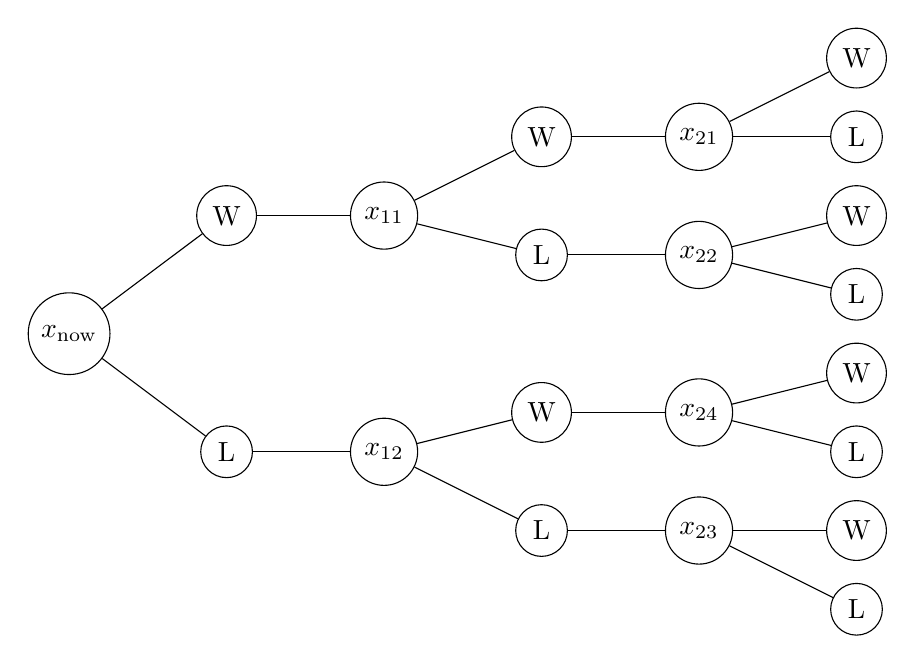
\begin{tikzpicture}
      \node (root) at (0,0) [circle,draw] {$x_{\mathrm{now}}$};

      \node (n1) at (2,1.5) [circle, draw] {W};
      \node (n2) at (2,-1.5) [circle, draw] {L};

      \draw (root) -- (n1);
      \draw (root) -- (n2);
      
      \node (n3) at (4,1.5) [circle, draw] {$x_{11}$};
      \node (n4) at (4,-1.5) [circle, draw] {$x_{12}$};

      \draw (n1) -- (n3);
      \draw (n2) -- (n4);

      \node (n5) at (6,2.5) [circle, draw] {W};
      \node (n6) at (6,1) [circle, draw] {L};
      \node (n7) at (6,-2.5) [circle, draw] {L};
      \node (n8) at (6,-1) [circle, draw] {W};

      \draw (n3) -- (n5);
      \draw (n3) -- (n6);
      \draw (n4) -- (n7);
      \draw (n4) -- (n8);
      
      \node (n9) at (8,2.5) [circle, draw] {$x_{21}$};
      \node (n10) at (8,1) [circle, draw] {$x_{22}$};
      \node (n11) at (8,-2.5) [circle, draw] {$x_{23}$};
      \node (n12) at (8,-1) [circle, draw] {$x_{24}$};

      \draw (n5) -- (n9) ;
      \draw (n6) -- (n10);
      \draw (n7) -- (n11);
      \draw (n8) -- (n12);

      \node (n13) at (10,3.5) [circle,draw]  {W};
      \node (n14) at (10,2.5) [circle,draw]  {L};
      \node (n15) at (10,1.5) [circle,draw]  {W};
      \node (n16) at (10,0.5) [circle,draw]  {L};
      \node (n17) at (10,-3.5) [circle,draw] {L};
      \node (n18) at (10,-2.5) [circle,draw] {W};
      \node (n19) at (10,-1.5) [circle,draw] {L};
      \node (n20) at (10,-0.5) [circle,draw] {W};

      \draw (n9) -- (n13);
      \draw (n9) -- (n14);
      \draw (n10) -- (n15);
      \draw (n10) -- (n16);
      \draw (n11) -- (n17);
      \draw (n11) -- (n18);
      \draw (n12) -- (n19);
      \draw (n12) -- (n20);
      
    \end{tikzpicture}
    \caption{The non-anticipativity constraints are violated in the first plot. Variables $x_{11},\ldots x_{14}$ share the identical history $\xi_{11}=\ldots = \xi_{14}=W$. Therefore, they must be identical. The tree structure below solves this problem by only introducing one variable for each distinct history.}
  \label{fig:violated-nonanticipativity}
\end{figure}